\documentclass{beamer}
% \documentclass[handout]{beamer}

\usepackage[linesnumbered,ruled,vlined ]{algorithm2e}
\usepackage{bm} %bold x in math mode
\usepackage{amsthm}
\definecolor{dred}{HTML}{730202}
\usepackage{tikz}
\usetikzlibrary{automata,arrows}
\usetikzlibrary{matrix}

\usepackage{latexsym,amsmath,amsfonts,amssymb,stmaryrd,mathtools,amsthm,ulem,multicol}
\usepackage[makeroom]{cancel}


\def\fe{Fuzzy Extractor\xspace}
\def\fes{Fuzzy Extractors\xspace}
\def\rfe{Reusable Fuzzy Extractor\xspace}
\def\ss{Secure Sketch\xspace}
\def\sss{Secure Sketches\xspace}
\def\dl{Digital Locker\xspace}
\def\dls{Digital Lockers\xspace}
\def\re{Randomness Extractor\xspace}
\newcommand{\gen}{\textit{Gen}\xspace}
\newcommand{\rep}{\textit{Rep}\xspace}
\newcommand{\sk}{\textit{SS}\xspace}
\newcommand{\rec}{\textit{Rec}\xspace}
\newcommand{\lock}{\textit{lock}\xspace}
\newcommand{\unlock}{\textit{unlock}\xspace}
\newcommand{\idealUnlock}{\textit{idealUnlock}\xspace}
\usepackage{ocgx}
\usepackage{mwe}
% \usepackage{pgfplots}
\usetikzlibrary{patterns}
\usepackage{appendixnumberbeamer}

 
\mode<presentation> {
\usetheme{Boadilla} %maybe
\usecolortheme{crane} %this
\setbeamertemplate{footline}[frame number] % To replace the footer line in all slides with a simple slide count uncomment this line
\setbeamertemplate{navigation symbols}{}
}

\usepackage{graphicx} % Allows including images
\usepackage{booktabs} % Allows the use of \toprule, \midrule and \bottomrule in tables

%----------------------------------------------------------------------------------------
%	TITLE PAGE
%----------------------------------------------------------------------------------------


\title{BioID: Fuzzy Extractor}

\author[]{Dalia Papuc\\Supervisor - Serge Vaudenay}
\institute{LASEC, EPFL
}
\date{\today} 


\begin{document}
{
\setbeamertemplate{footline}{} 
\begin{frame}[noframenumbering]
\titlepage % Print the title page as the first slide
\end{frame}
}

%------------------------------------------------
\begin{frame}{Introduction}
User authentication using biometric features is widely used, e.g., unlocking your phone this morning~\pause

\begin{figure}
    \centering
    \begin{tikzpicture}[>=stealth', shorten >=1pt, auto, node distance=4cm and 3cm, scale=.75, transform shape, align=center,state/.style={circle, draw, minimum size=0.75cm,font=\small}]

% \visible<2->{
    \node[label=below:Alice's finger-vein pattern] (A) {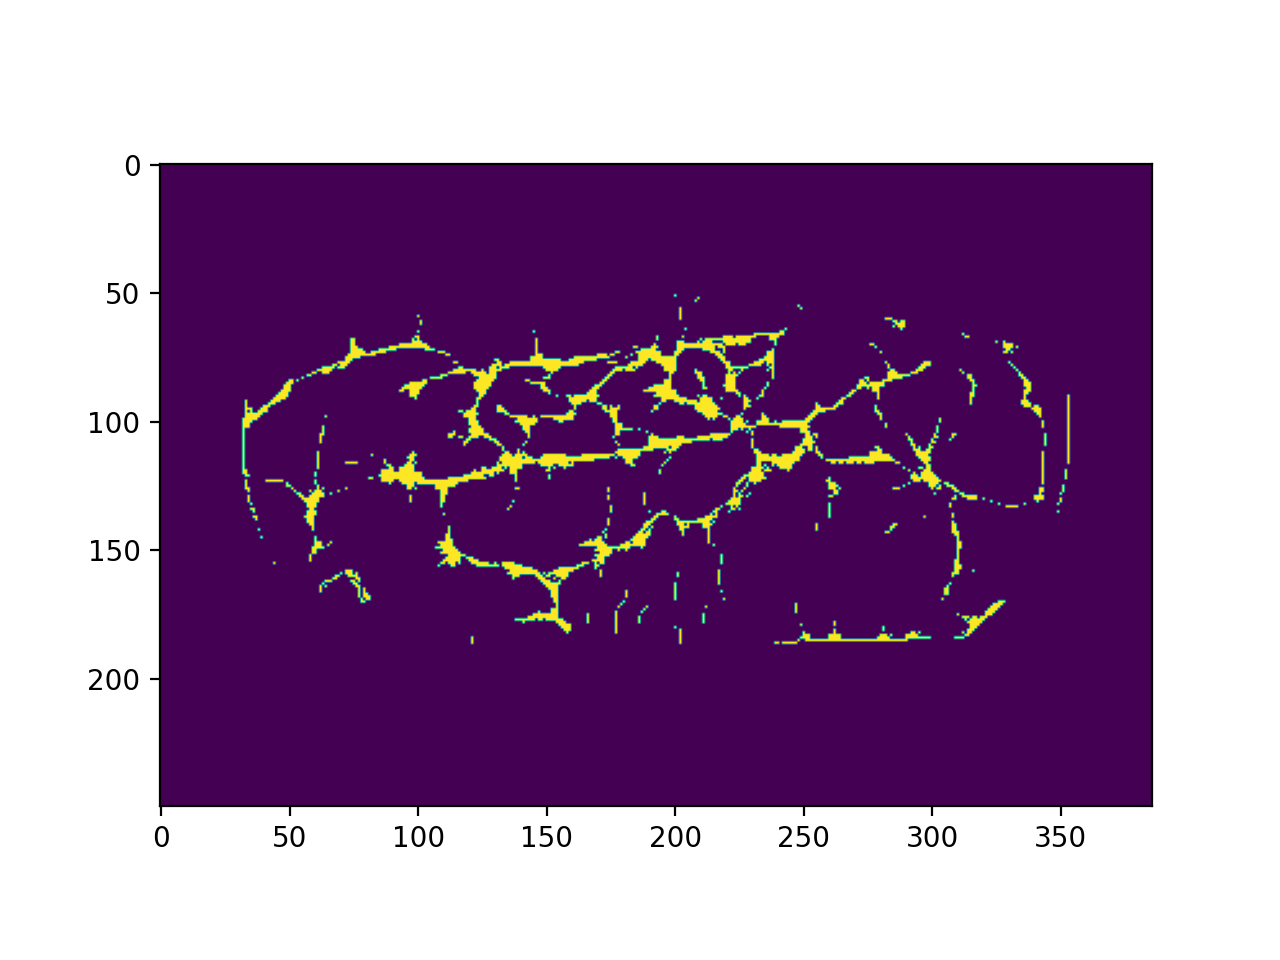
\includegraphics[width=.7\textwidth]{z.png}};%}
\end{tikzpicture}
\end{figure}
\end{frame}
%------------------------------------------------
\begin{frame}{\fes}
    \fes convert noisy non-uniform inputs into reliably reproducible, uniform random strings\\~\pause
    
\begin{figure}
    \centering
    \begin{tikzpicture}[>=stealth', shorten >=1pt, auto, node distance=2cm and 1cm, scale=.75, transform shape, align=center,state/.style={circle, draw, minimum size=0.75cm,font=\small}]

\visible<2>{
  \node[text width=5.5cm] (B) {a reading of the biometric feature (the model)};
  \node[state,rectangle,minimum width=2.3cm,yshift=0cm, below of=B]           (A){Generate (\gen)};
  \node[text width=5.5cm,below of=A,yshift=0cm] (C) {a uniform random string $r$ \& a public helper string $p$};
  
  \node[text width=5.5cm,right of =B, xshift=4.5cm] (D) {the helper string $p$ \& another reading of the same biometric feature (a probe)};
  \node[state,rectangle,minimum width=2.3cm,yshift=0cm, below of=D]           (E){Reproduce (\rep)};
  \node[text width=5.5cm,below of=E,yshift=0cm] (F) {the uniform random string $r$ or $\bot$};  
  
    \path[->,draw]
    (B) edge node[] {} (A)
    (A) edge node[] {} (C)
    (D) edge node[] {} (E)
    (E) edge node[] {} (F);
}
\visible<3>{
  \node[text width=5.5cm] (B) {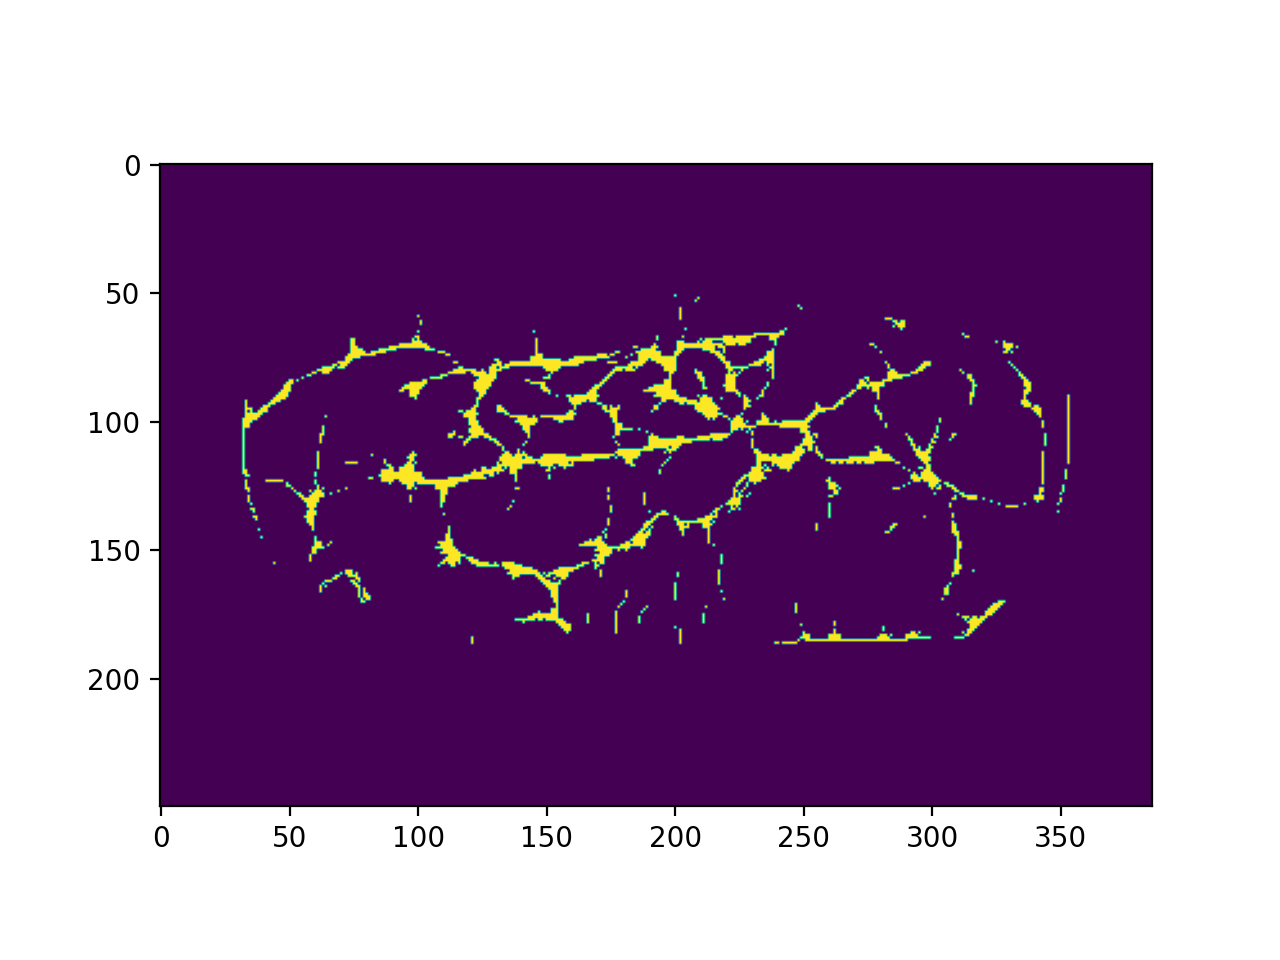
\includegraphics[width=.6\textwidth]{z.png}};
  \node[state,rectangle,minimum width=2.3cm,yshift=0cm, below of=B]           (A){Generate (\gen)};
  \node[text width=5.5cm,below of=A,yshift=0cm] (C) { $r, p$};
  
  \node[text width=5.5cm,right of =B, xshift=4.5cm] (D) {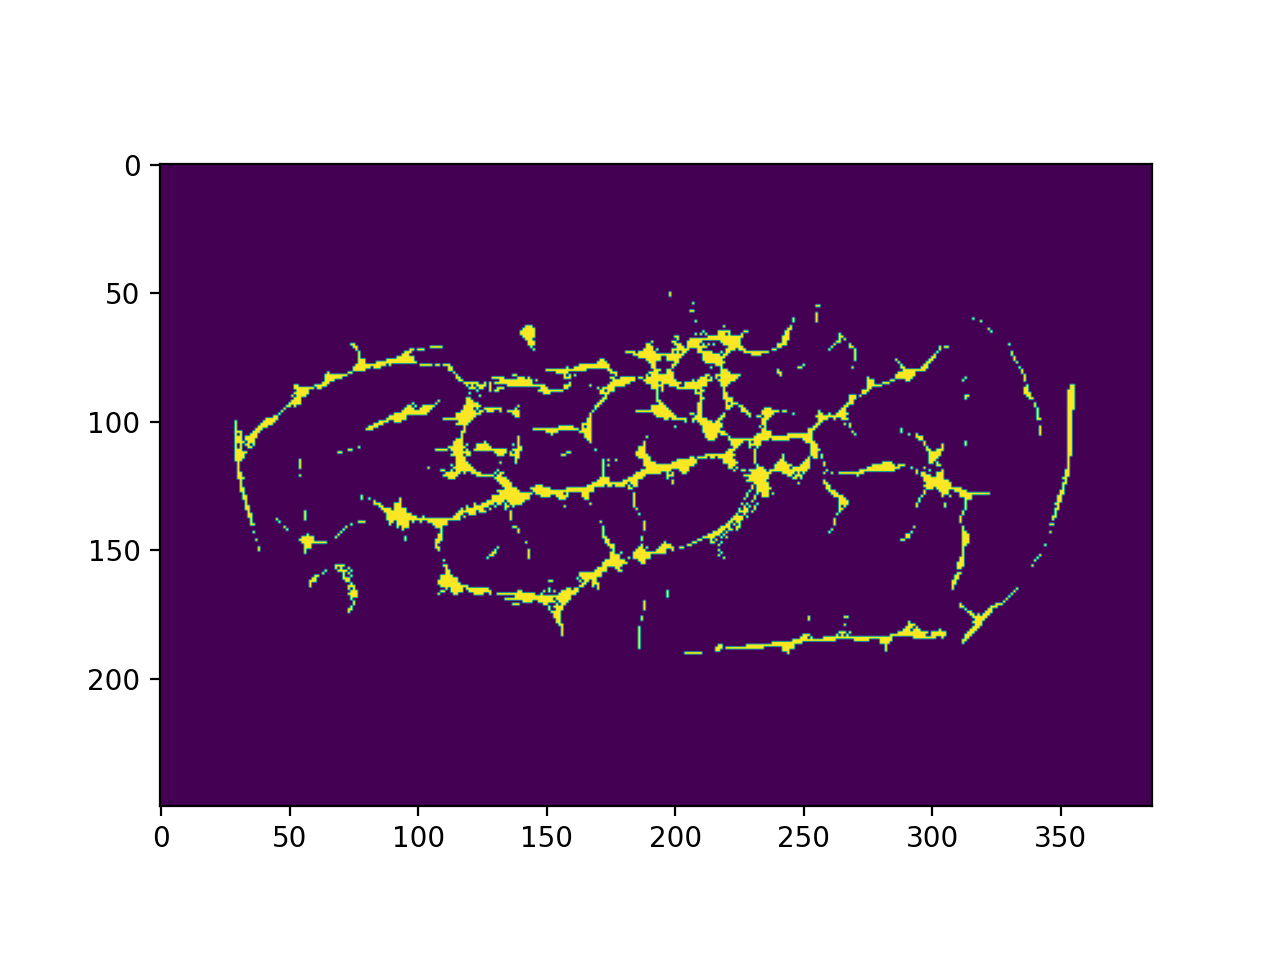
\includegraphics[width=.6\textwidth]{z2.png}, $p$};
  \node[state,rectangle,minimum width=2.3cm,yshift=0cm, below of=D]           (E){Reproduce (\rep)};
  \node[text width=5.5cm,below of=E,yshift=0cm] (F) {$r$};  
  
    \path[->,draw]
    (B) edge node[] {} (A)
    (A) edge node[] {} (C)
    (D) edge node[] {} (E)
    (E) edge node[] {} (F);
}
\visible<4>{
  \node[text width=5.5cm] (B) {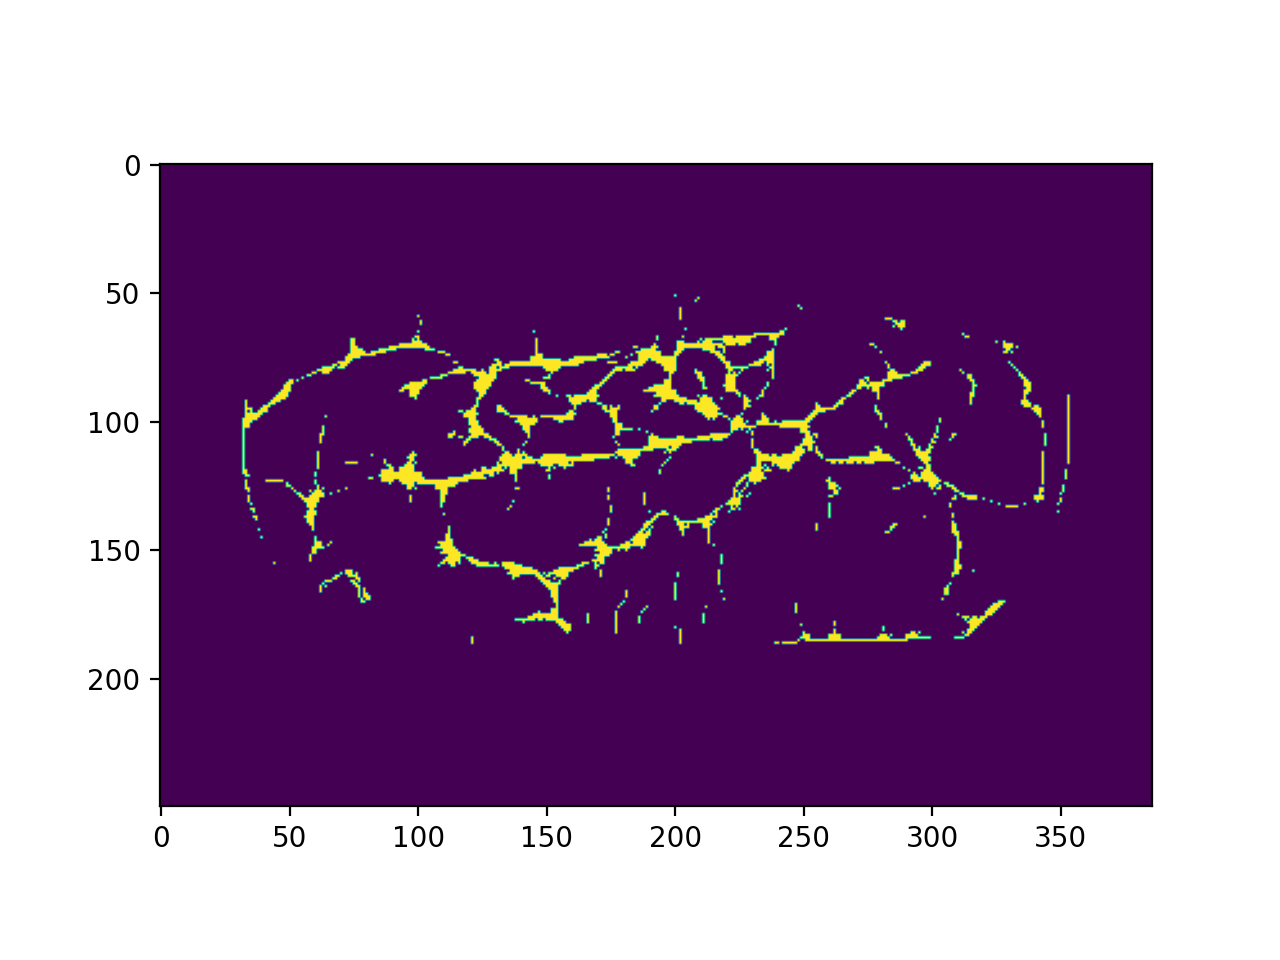
\includegraphics[width=.6\textwidth]{z.png}};
  \node[state,rectangle,minimum width=2.3cm,yshift=0cm, below of=B]           (A){Generate (\gen)};
  \node[text width=5.5cm,below of=A,yshift=0cm] (C) { $r, p$};
  
  \node[text width=5.5cm,right of =B, xshift=4.5cm] (D) {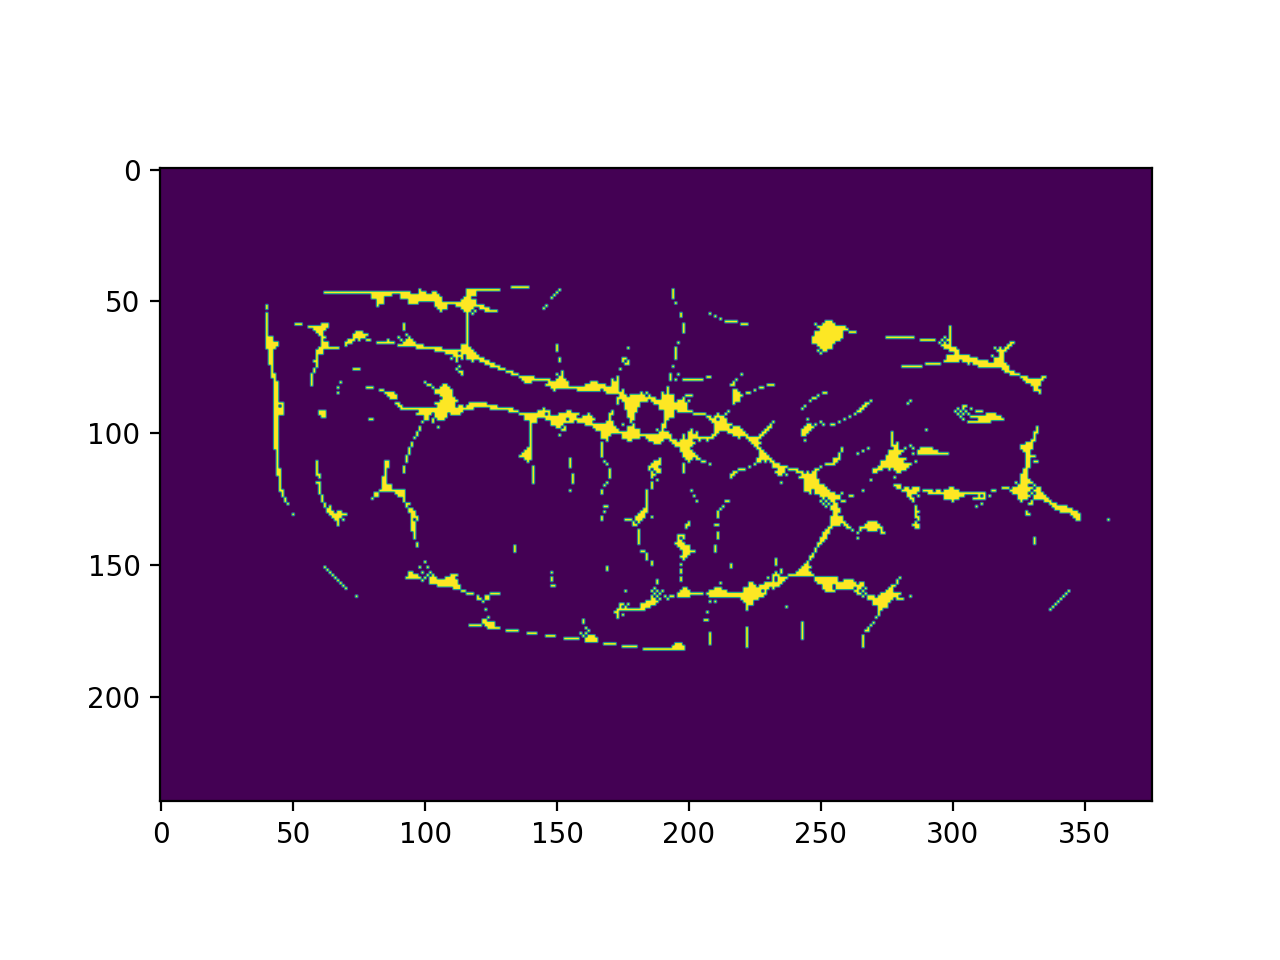
\includegraphics[width=.6\textwidth]{q.png}, $p$};
  \node[state,rectangle,minimum width=2.3cm,yshift=0cm, below of=D]           (E){Reproduce (\rep)};
  \node[text width=5.5cm,below of=E,yshift=0cm] (F) {$\bot$};  
  
    \path[->,draw]
    (B) edge node[] {} (A)
    (A) edge node[] {} (C)
    (D) edge node[] {} (E)
    (E) edge node[] {} (F);
}
\end{tikzpicture}
\end{figure}\pause
    
    E.g., \gen at enrolment and \rep to authenticate Alice whenever desired
    
\end{frame}
%------------------------------------------------
\begin{frame}{Challenges}
% \only<1-2>{
   \begin{enumerate}
       \item Find a suitable \fe construction\\~\pause 
       
       \item Data has noise
   \end{enumerate} 
%  }
 \end{frame}
 \begin{frame}{Outline}
% \only<3->{
% \setcounter{beamerpauses}{2}
   \begin{enumerate}
       \item Find a suitable \fe construction~\pause
    \begin{enumerate}
        \item Wish-list~\pause
        \item The construction~\pause
        \item Parameter estimation\\~\pause
    \end{enumerate}
       \item Data has noise~\pause
       \begin{enumerate}
           \item Access to the model \& probe~\pause
           \item Access to multiple instances of \rep~\pause
           \item Access to a single instance of \rep~\pause
            \begin{enumerate}
                \item Alignment methods (4)~\pause
                \item Evaluation
            \end{enumerate}
       \end{enumerate}    
   \end{enumerate} 
% } 
\end{frame}
%------------------------------------------------
\begin{frame}{Preliminaries}
\textit{Metric space:} set $\mathcal{M}$ with a distance function $dis: \mathcal{M} \times \mathcal{M} \xrightarrow{} \mathbb{R}^{+}$ e.g., Hamming metric, set difference metric, edit metric\\~\pause

\textit{Hamming metric:} $\mathcal{M}=\mathcal{F}^n$, for some alphabet $\mathcal{F}$, and $dis(w,w')$ the number of positions in which the strings $w$ and $w'$ differ\\~\pause

% adv needs to guess most likely value
Probability adversary predicts a RV (e.g., guesses secret): best strategy guess most likely value\\
\textit{Predictability} of RV $A$: $\max_a\Pr[A=a]$\\~\pause

Correspondingly, \textit{min-entropy}: $\mathbf{H}_\infty(A)=-\log(\max_a\Pr[A=a])$\\
Min-entropy of a distribution tells how many nearly uniform random bits can be extracted from it

\end{frame}
%------------------------------------------------
\begin{frame}{\fe}{An ($\mathcal{M},m,\ell,t,\epsilon$)-\fe with error $\delta$}
A pair of randomised procedures, \gen and \rep:\\~\pause

\textit{Generate} (\gen): takes as input $w \in \mathcal{M}$, it outputs an extracted string $r \in \{0,1\}^\ell$, and a (public) helper string $p\in\{0,1\}^*$\\~\pause

\textit{Reproduce} (\rep): takes as input $w' \in \mathcal{M}$ and a bit string $p\in\{0,1\}^*$\\~\pause
% \qquad Output: $r$\\

\textit{Correctness:} $\forall (w,w')$ s.t.\ $dis(w,w')\leq t$, for $\gen(w)=(R,P)$, then $\rep(w',P)=R$  with probability (over the coins of \gen, \rep) at least $1-\delta$. If $dis(w,w') > t$, no guarantees\\~\pause

\textit{Security:}  $\forall$ distribution $W$ on $\mathcal{M}$ of min-entropy $m$, the string $R$ is nearly uniform even for those who observe $P$: if $\gen(w)=(R,P)$, then
$$\mathbf{SD}((R,P),(U_\ell,P)) \leq \epsilon \footnote{$U_\ell$: uniform distribution on $\ell-$bit binary strings; $\mathbf{SD}$: statistical distance}$$
\end{frame}
%------------------------------------------------
\begin{frame}{Outline}
   \begin{enumerate}
   \item Find a suitable \fe construction
\begin{enumerate}
    \item \textbf{Wish-list}
    \item The construction
    \item Parameter estimation\\
\end{enumerate}
   \item Data has noise
   \begin{enumerate}
       \item Access to the model \& probe
       \item Access to multiple instances of \rep
       \item Access to a single instance of \rep
        \begin{enumerate}
            \item Alignment methods (4)
            \item Evaluation
        \end{enumerate}
   \end{enumerate}    
\end{enumerate} 
\end{frame}
%------------------------------------------------
\begin{frame}{Wish-list}
    \begin{enumerate}
        \item Use the finger-vein pattern as input
    \end{enumerate}
\end{frame}
%------------------------------------------------
\begin{frame}{Sketch-then-Extract}
A common approach in \fe constructions: \ss and \re\\~\pause

\ss: recovers original $w$ from any nearby value $w'$\pause

\begin{figure}
    \centering
    \begin{tikzpicture}[>=stealth', shorten >=1pt, auto, node distance=2cm and 1cm, scale=.75, transform shape, align=center,state/.style={circle, draw, minimum size=0.75cm,font=\small}]

\visible<3>{
  \node[text width=5.5cm] (B) {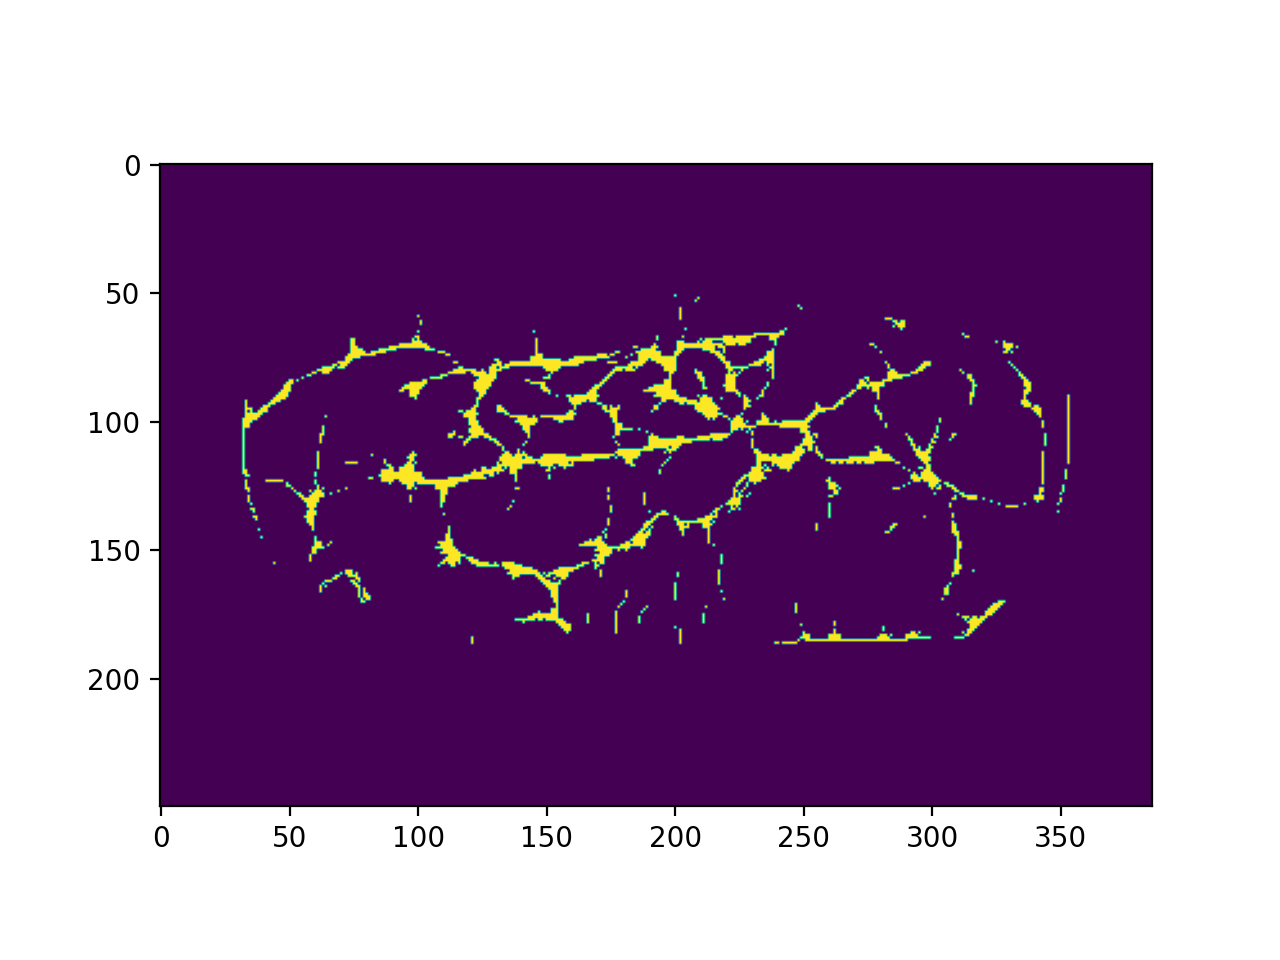
\includegraphics[width=.6\textwidth]{z.png}};
  \node[state,rectangle,minimum width=2.3cm,yshift=0cm, below of=B]           (A){Sketch (\sk)};
  \node[text width=5.5cm,below of=A,yshift=0cm] (C) { bit-string $s$};
  
  \node[text width=5.5cm,right of =B, xshift=4.5cm] (D) {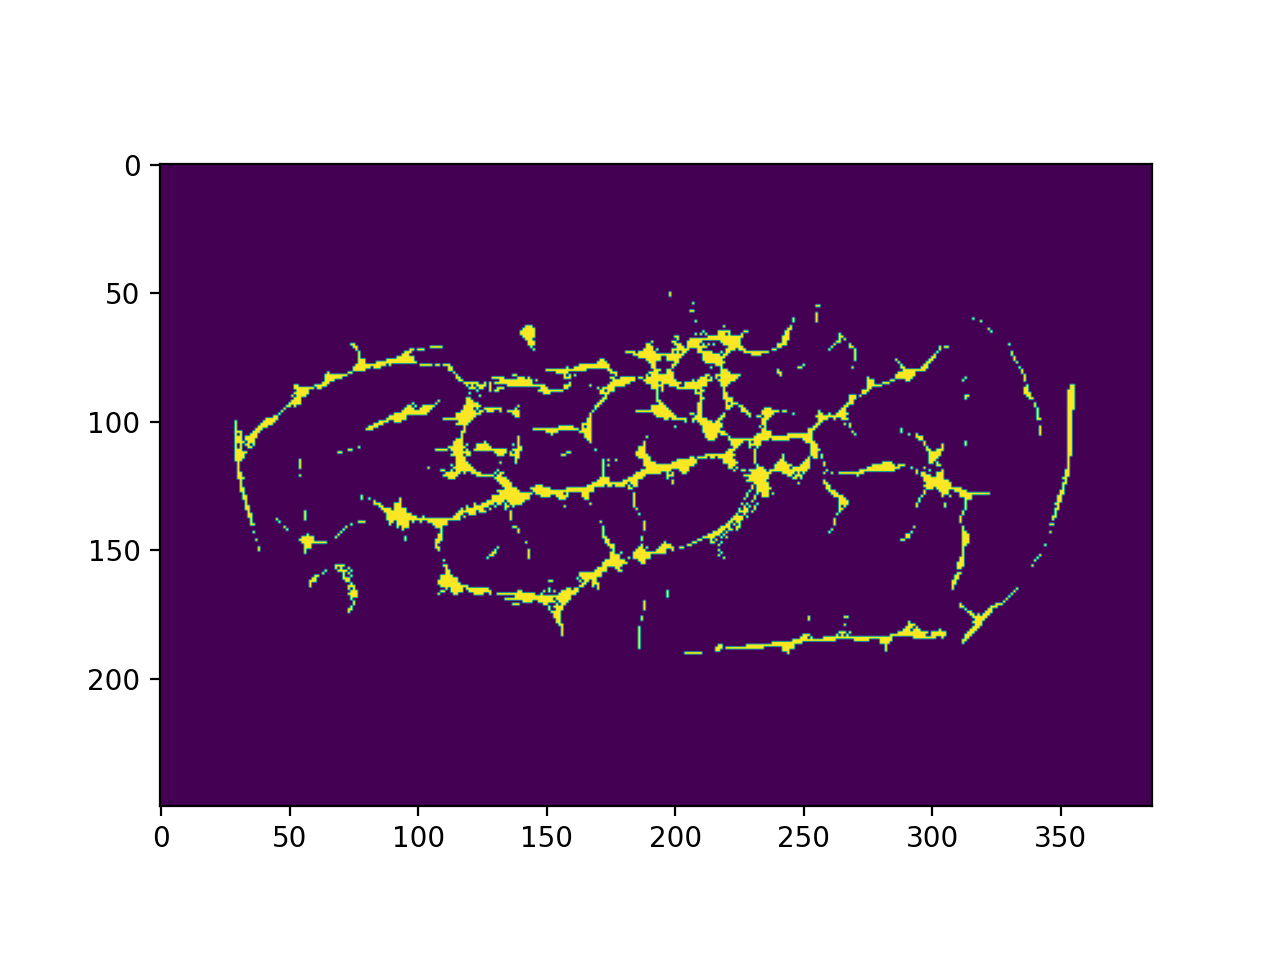
\includegraphics[width=.6\textwidth]{z2.png}, $s$};
  \node[state,rectangle,minimum width=2.3cm,yshift=0cm, below of=D]           (E){Recover (\rec)};
  \node[text width=5.5cm,below of=E,yshift=0cm] (F) {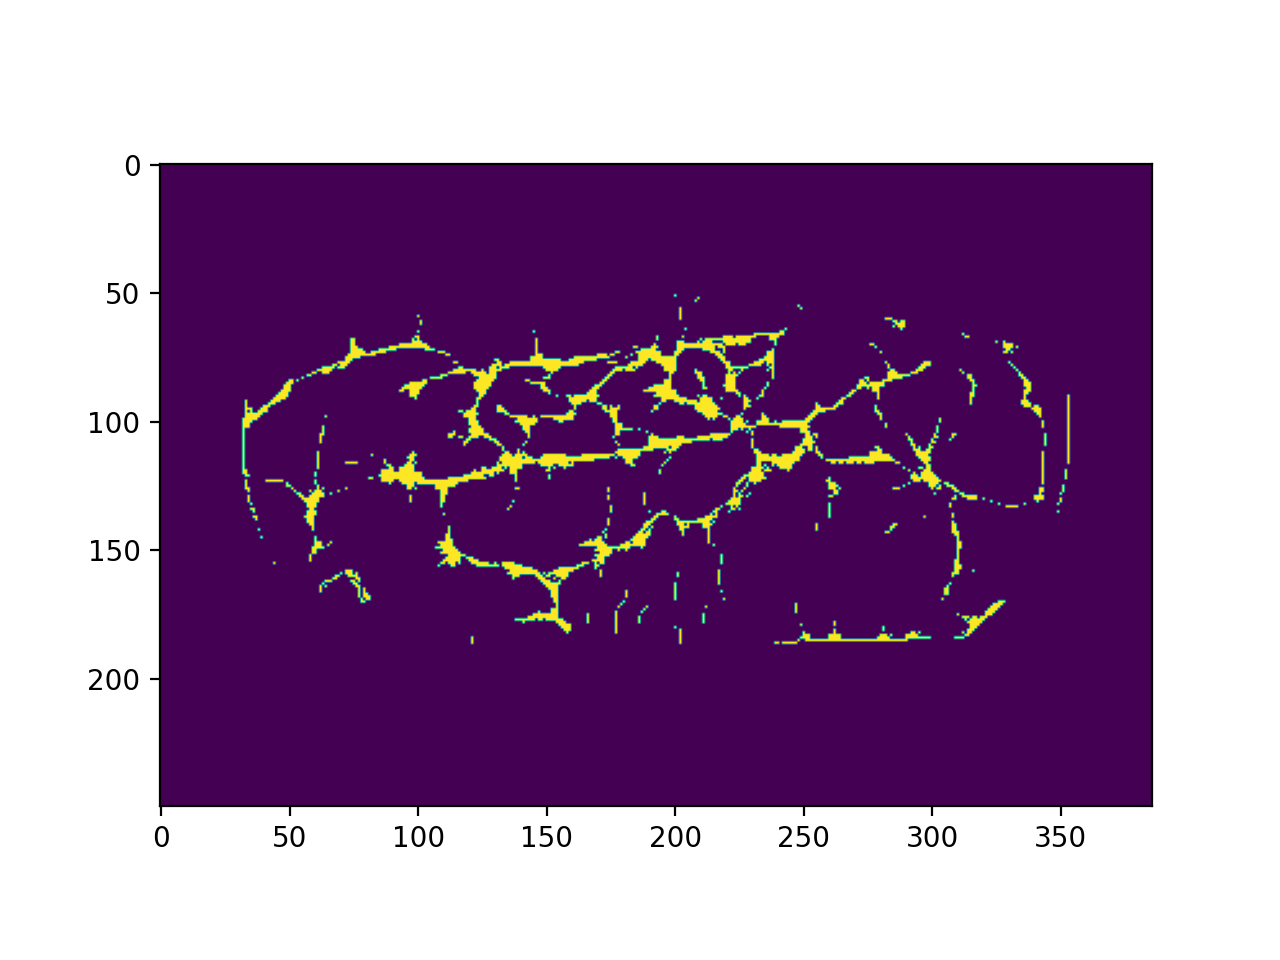
\includegraphics[width=.6\textwidth]{z.png}};  
  
    \path[->,draw]
    (B) edge node[] {} (A)
    (A) edge node[] {} (C)
    (D) edge node[] {} (E)
    (E) edge node[] {} (F);
}
\visible<4>{
  \node[text width=5.5cm] (B) {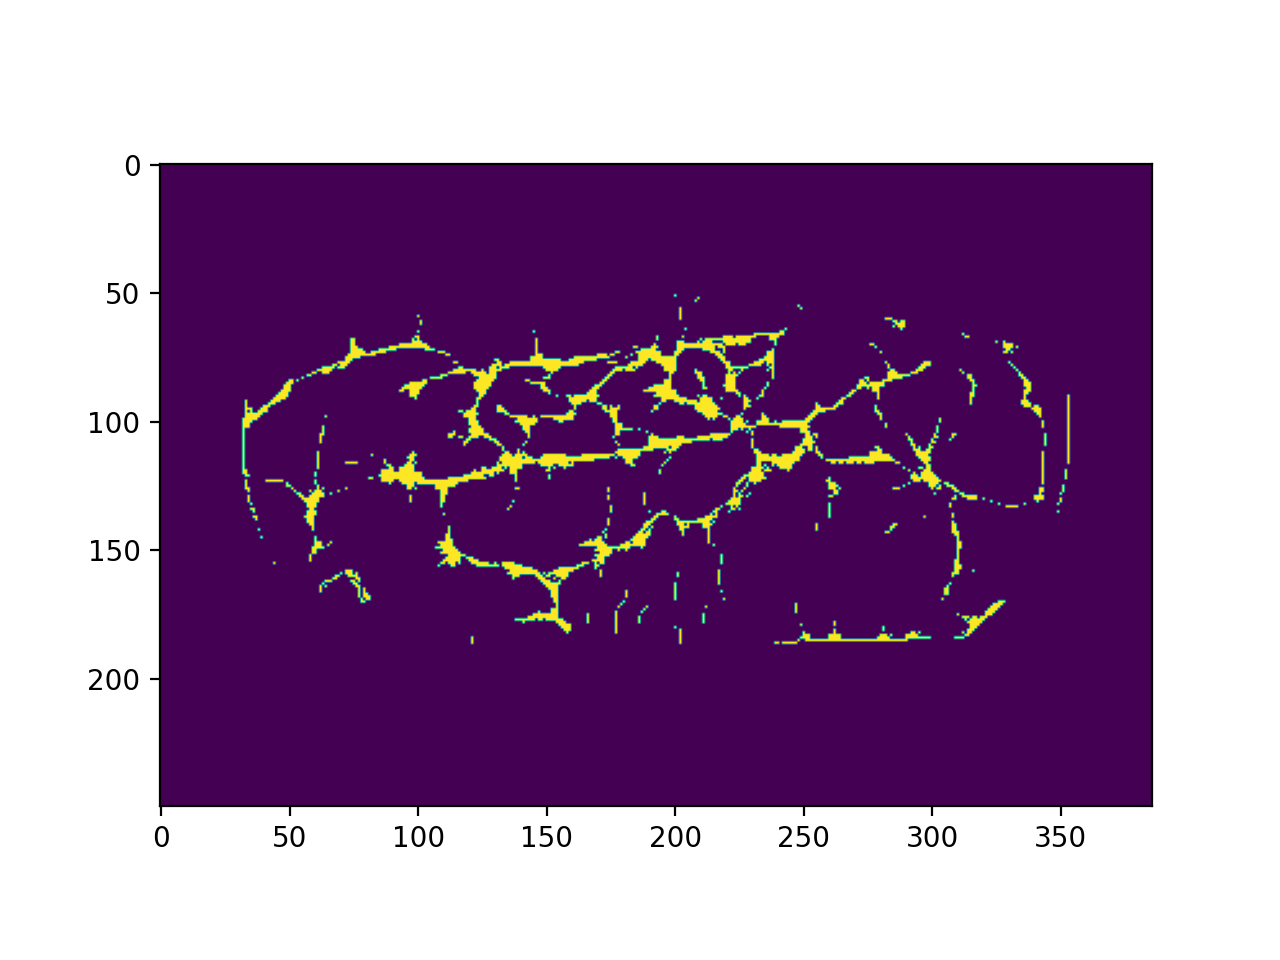
\includegraphics[width=.6\textwidth]{z.png}};
  \node[state,rectangle,minimum width=2.3cm,yshift=0cm, below of=B]           (A){Sketch (\sk)};
  \node[text width=5.5cm,below of=A,yshift=0cm] (C) { bit-string $s$};
  
  \node[text width=5.5cm,right of =B, xshift=4.5cm] (D) {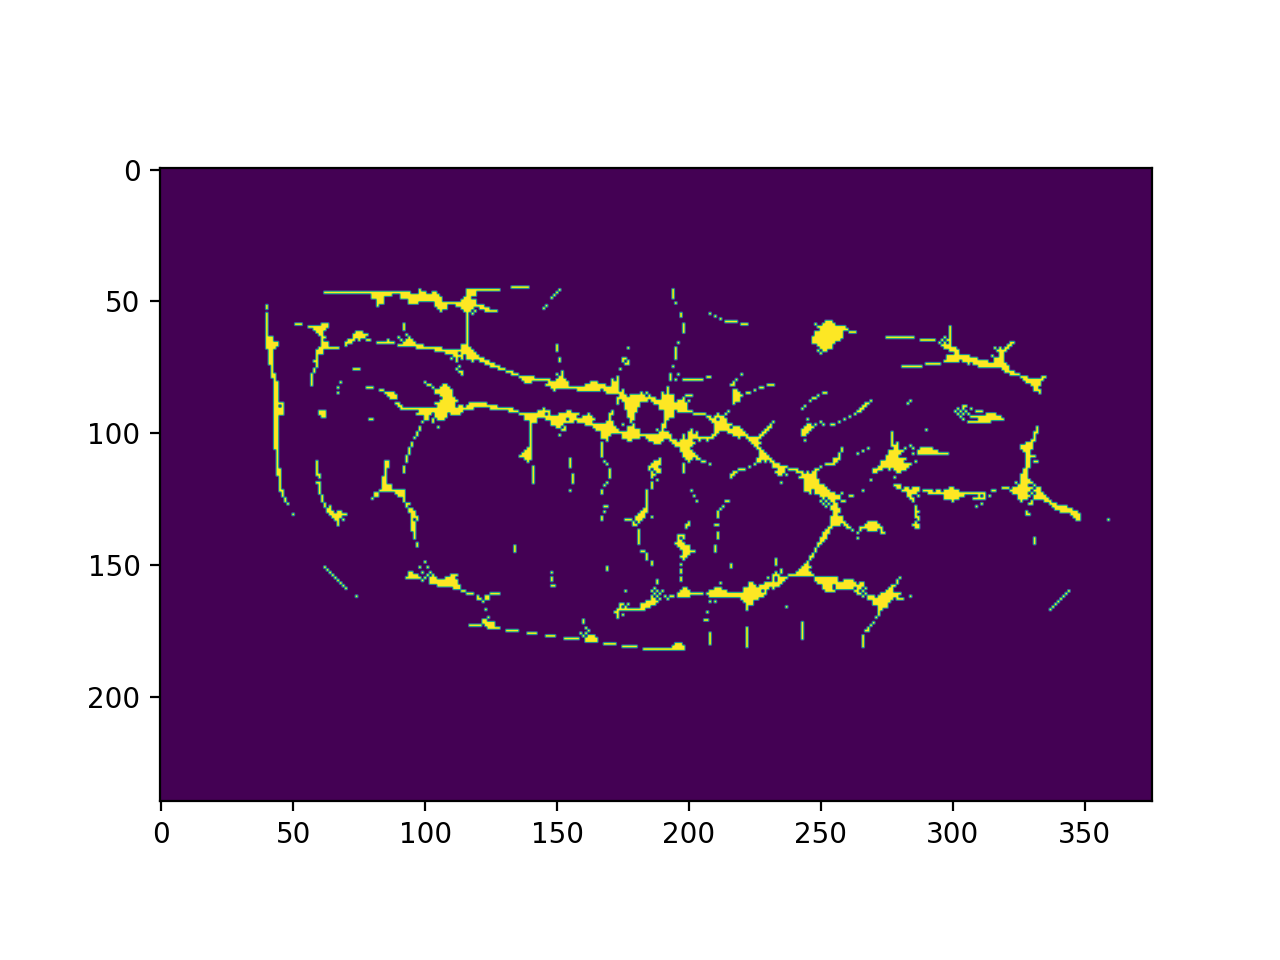
\includegraphics[width=.6\textwidth]{q.png}, $s$};
  \node[state,rectangle,minimum width=2.3cm,yshift=0cm, below of=D]           (E){Recover (\rec)};
  \node[text width=5.5cm,below of=E,yshift=0cm] (F) {$\bot$};  
  
    \path[->,draw]
    (B) edge node[] {} (A)
    (A) edge node[] {} (C)
    (D) edge node[] {} (E)
    (E) edge node[] {} (F);
}
\end{tikzpicture}
\end{figure}\pause

\re: run on $w$ to produce uniform bits%\\~\pause

\end{frame}
%------------------------------------------------
%------------------------------------------------
\begin{frame}{Wish-list}
    \begin{enumerate}
        \item Use the finger-vein pattern as input\\~
        \item Construction is hard to invert [FMR13,YY18]
    \end{enumerate}
\end{frame}
%------------------------------------------------
\begin{frame}{Reusability}
\gen is called $\rho$ times on \textit{correlated} readings $w^1 \dots w^\rho$ of the same source, producing $(r^1,p^1),\dots, (r^\rho,p^\rho)$ \\~\pause

\fe constructions leak information on input data [B04]\\~\pause % when \gen is called multiple times on different readings of the same source \\~\pause

Security should hold for each $r^i$ even when $p^1 \dots p^\rho$ and all $r^j$, $j\neq i$, are known\\~\pause

$\implies$ Consider constructions that provide reusability\\~\pause

Correlated readings of the same source: arbitrary or shift\\~\pause


$\implies$ Consider arbitrary correlations
\end{frame}
%------------------------------------------------
\begin{frame}{Wish-list}
    \begin{enumerate}
        \item Use the finger-vein pattern as input\\~
        \item Construction is hard to invert [FMR13,YY18]\\~
        \item Construction provides reusability\\~
        \item Arbitrary correlations for multiple readings of the same source 
    \end{enumerate}
\end{frame}
%------------------------------------------------

%------------------------------------------------
\begin{frame}{Outline}
   \begin{enumerate}
   \item Find a suitable \fe construction
\begin{enumerate}
    \item Wish-list
    \item \textbf{The construction}
    \item Parameter estimation\\
\end{enumerate}
   \item Data has noise
   \begin{enumerate}
       \item Access to the model \& probe
       \item Access to multiple instances of \rep
       \item Access to a single instance of \rep
        \begin{enumerate}
            \item Alignment methods (4)
            \item Evaluation
        \end{enumerate}
   \end{enumerate}    
\end{enumerate} 
\end{frame}
%------------------------------------------------
\begin{frame}{The construction [CFP$^+$16]}

Checks all boxes on the wish-list\\~\pause

Uses \dl: computationally secure symmetric-encryption scheme\pause
\begin{figure}
    \centering
    \begin{tikzpicture}[>=stealth', shorten >=1pt, auto, node distance=2cm and 1cm, scale=.75, transform shape, align=center,state/.style={circle, draw, minimum size=0.75cm,font=\small}]

\visible<3>{
  \node[text width=5.5cm] (B) {$key, val$};
  \node[state,rectangle,minimum width=2.3cm,yshift=0cm, below of=B]           (A){$\lock$};
  \node[text width=5.5cm,below of=A,yshift=0cm] (C) {$c$};
  
  \node[text width=5.5cm,right of =B, xshift=4.5cm] (D) {$key,c$};
  \node[state,rectangle,minimum width=2.3cm,yshift=0cm, below of=D]           (E){$\unlock$};
  \node[text width=5.5cm,below of=E,yshift=0cm] (F) {$val$};  
  
    \path[->,draw]
    (B) edge node[] {} (A)
    (A) edge node[] {} (C)
    (D) edge node[] {} (E)
    (E) edge node[] {} (F);
}
\visible<4->{
  \node[text width=5.5cm] (B) {$key, val$};
  \node[state,rectangle,minimum width=2.3cm,yshift=0cm, below of=B]           (A){$\lock$};
  \node[text width=5.5cm,below of=A,yshift=0cm] (C) {$c$};
  
  \node[text width=5.5cm,right of =B, xshift=4.5cm] (D) {$key',c$};
  \node[state,rectangle,minimum width=2.3cm,yshift=0cm, below of=D]           (E){$\unlock$};
  \node[text width=5.5cm,below of=E,yshift=0cm] (F) {$\bot$};  
  
    \path[->,draw]
    (B) edge node[] {} (A)
    (A) edge node[] {} (C)
    (D) edge node[] {} (E)
    (E) edge node[] {} (F);
}

\end{tikzpicture}
\end{figure}
\pause

Sample-then-Lock approach:\pause
\begin{itemize}
    \item Generate a fresh random string $r$\pause
    \item Lock $r$ using parts of $w$ in an error-tolerant way\\~\pause
\end{itemize}

Requires sources with high-entropy samples
    
\end{frame}
%------------------------------------------------
\begin{frame}{Assumptions on source}

    Commonly require $w$ to have \textit{sufficient min-entropy}. Now:\\~\pause

    Source $w$ with \textit{high entropy sample}: for some known $k$, sub-string formed by bits at $k$ randomly chosen positions in $w$ is unguessable\\~\pause

    Sampling preserves entropy rate \& low-entropy sources may exhibit high-entropy samples (relative to the length of the string) \\~\pause   
    % , e.g., an image of the iris

\textcolor{dred}{Challenge:} Finger-vein pattern has considerably more $0$s than $1$s\\~\pause

\textcolor{dred}{Approach:} Use the biometric hash of the finger-vein pattern instead % to obtain an equal ratio of $-1$s and $1$s
\end{frame}
%------------------------------------------------
\begin{frame}{Pseudocode [CFP$^+$16, SSF18]}
    \begin{multicols}{2}
\gen

\textbf{Input:} $w = w_1,\dots,w_n$ 

Sample $r \xleftarrow{\$} \{0,1\}^\ell$

For $i = 1,\dots, f$:

        \quad Choose random $1 \leq j_{i,1},\dots, j_{i,k} \leq n$
        
        \quad Set $v_i = w_{j_{i,1}},\dots, w_{j_{i,k}}$ 
        
        \quad Set $c_i = \lock(v_i, r)$
        
        \quad Set $p_i = c_i, (j_{i,1},\dots, j_{i,k})$

\textbf{Output:} $(r,p)$, where $p = p_1 \dots p_f$.

\columnbreak
\rep

\textbf{Input:} $(w' = w'_1,\dots,w'_n, p = p_1 \dots p_f)$ 

For $i = 1,\dots, f$:

        \quad Parse $p_i = c_i, (j_{i,1},\dots, j_{i,k})$
        
        \quad Set $v'_i = w'_{j_{i,1}},\dots, w'_{j_{i,k}}$ 
        
        \quad Set $r_i = \unlock(v'_i, c_i)$
        
        \quad If $r_i \neq \bot$:
        
        \qquad\textbf{Output:}  $r_i$

\textbf{Output:} $\bot$.

\end{multicols}\pause
\begin{multicols}{2}
\small
$c_i = \lock(v_i,r) = nonce, HMAC(nonce, v_i) \oplus (0^{256}||r)$
\columnbreak

$z_i = \unlock(v_i',c_i) = HMAC(c1_i, v'_i) \oplus c2_i$ 

If $z_i$ has a prefix of $0^{256}$:

    \quad Return suffix $r$
\end{multicols}
\end{frame}
%------------------------------------------------
\begin{frame}{Outline}
   \begin{enumerate}
   \item Find a suitable \fe construction
\begin{enumerate}
    \item Wish-list
    \item The construction
    \item \textbf{Parameter estimation}\\
\end{enumerate}
   \item Data has noise
   \begin{enumerate}
       \item Access to the model \& probe
       \item Access to multiple instances of \rep
       \item Access to a single instance of \rep
        \begin{enumerate}
            \item Alignment methods (4)
            \item Evaluation
        \end{enumerate}
   \end{enumerate}    
\end{enumerate} 
\end{frame}
%------------------------------------------------
\begin{frame}{Parameter estimation (I)}
The number of \dls $f$ and the sample size $k$ via: 

$$ 1- \left(1 - \left(1 - mean\;error\;rate \right)^k\right)^f = correctness\;target$$\\~\pause
% where the $correctness\;target$ is e.g., the desired True Positive Rate ($TPR$)

% To compute the $mean\;error\;rate$ we consider intraclass comparisons. We compute the Hamming distance between two biometric hashes of the same finger and obtain a 

$mean\;error\;rate = 0.418643$ for intraclass comparisons\\~\pause

When $k=40$, we need $\approx f=3.2\times10^{9}$ lockers to obtain a target correctness of $70\%$ \\~\pause

\textcolor{dred}{Warning: 2-users dataset!} Yet what if these results were valid?

\end{frame}
%------------------------------------------------
\begin{frame}{Parameter estimation (II)}
To obtain higher security, we can:\\~
\begin{enumerate}
    \item increase the number of lockers\label{it:sec1}\\~\pause
    \item decrease the target correctness rate\label{it:sec11}\\~\pause
    \item reduce the mean error rate\label{it:sec2}\\~\pause
    \item consider strong-authentication \label{it:sec22}\\~\pause
    \item opt for a different scheme\label{it:sec3}
\end{enumerate}
  
\end{frame}
%------------------------------------------------

\begin{frame}{Outline}
   \begin{enumerate}
   \item Find a suitable \fe construction
\begin{enumerate}
    \item Wish-list
    \item The construction
    \item Parameter estimation\\
\end{enumerate}
   \item \textbf{Data has noise}
   \begin{enumerate}
       \item Access to the model \& probe
       \item Access to multiple instances of \rep
       \item Access to a single instance of \rep
        \begin{enumerate}
            \item Alignment methods (4)
            \item Evaluation
        \end{enumerate}
   \end{enumerate}    
\end{enumerate} 
\end{frame}
%------------------------------------------------

\begin{frame}{Outline}
   \begin{enumerate}
   \item Find a suitable \fe construction
\begin{enumerate}
    \item Wish-list
    \item The construction
    \item Parameter estimation\\
\end{enumerate}
   \item Data has noise
   \begin{enumerate}
       \item \textbf{Access to the model \& probe}
       \item Access to multiple instances of \rep
       \item Access to a single instance of \rep
        \begin{enumerate}
            \item Alignment methods (4)
            \item Evaluation
        \end{enumerate}
   \end{enumerate}    
\end{enumerate} 
\end{frame}
%------------------------------------------------
\begin{frame}{Access to the model \& probe}
Provides the most opportunities for the transformations possible on the probe \\~\pause

\begin{figure}
    \centering
    \begin{tikzpicture}[>=stealth', shorten >=1pt, auto, node distance=2cm and 1cm, scale=.75, transform shape, align=center,state/.style={circle, draw, minimum size=0.75cm,font=\small}]

\visible<2->{
\node[text width=5.5cm, xshift=-1cm,label=below:Model] (A) {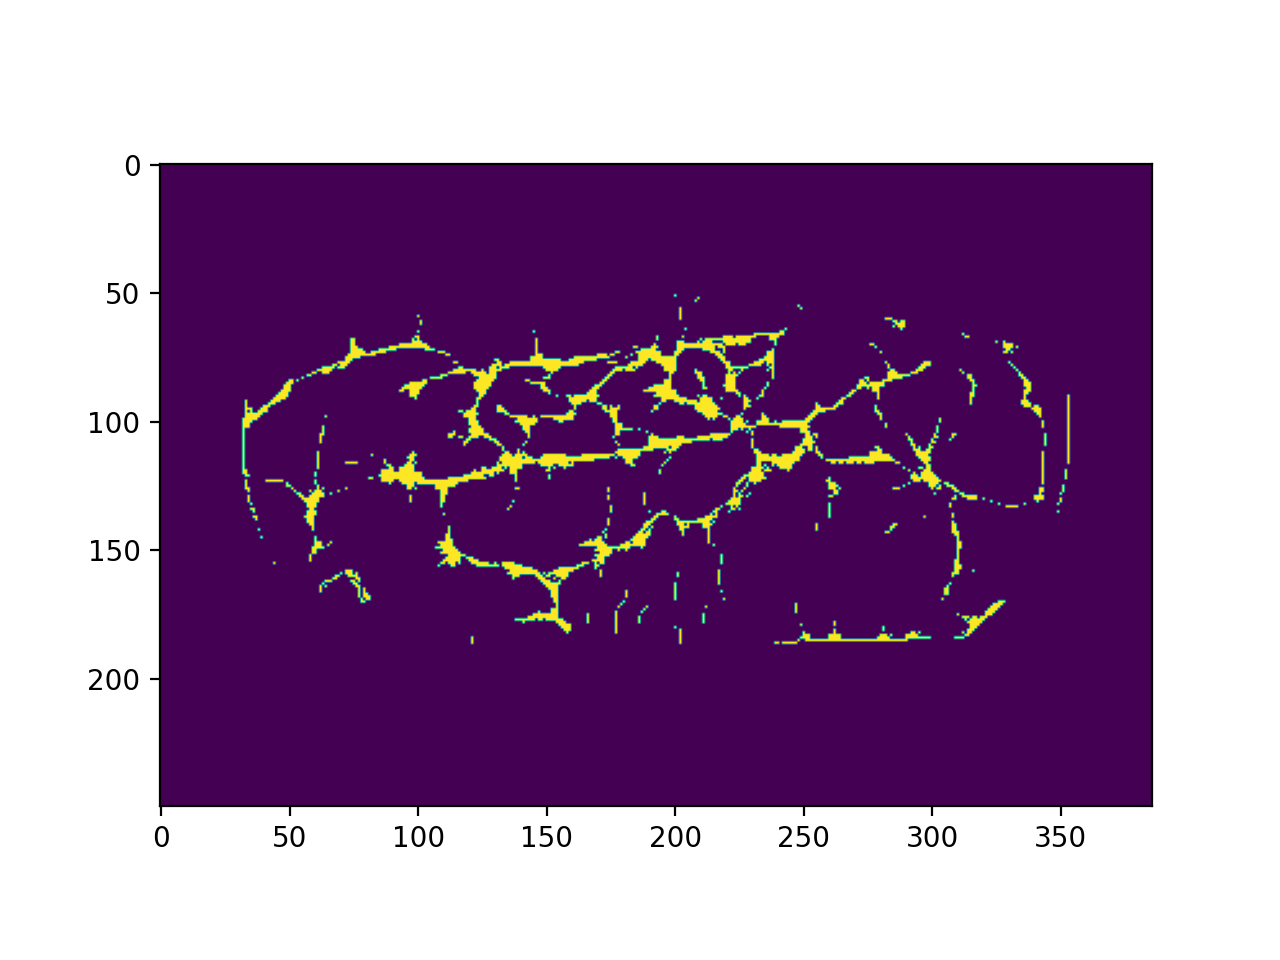
\includegraphics[width=.6\textwidth]{z.png}};
\node[text width=5.5cm,right of =A, xshift=1.5cm, label=below:Probe] (B) {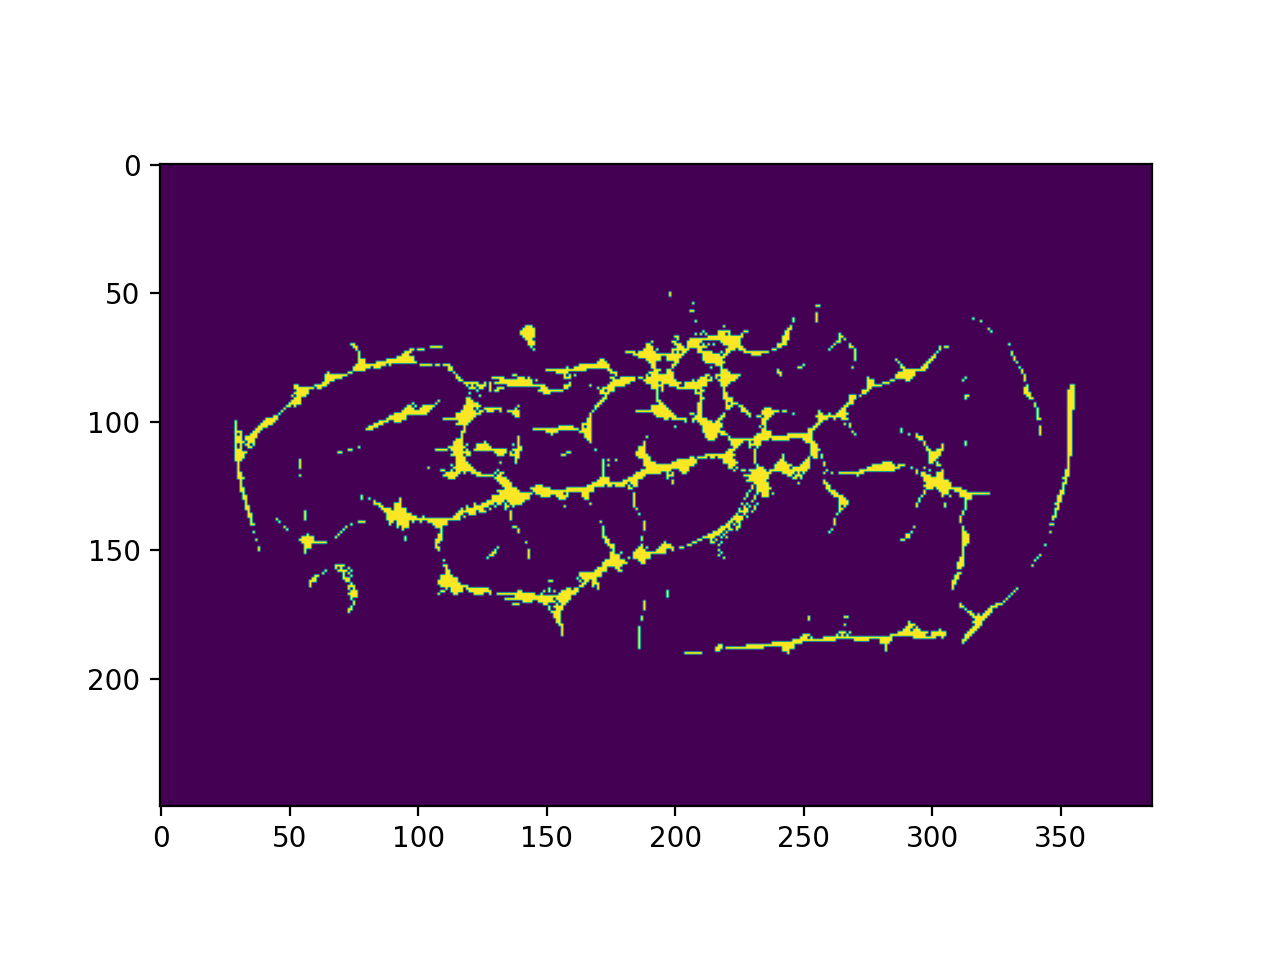
\includegraphics[width=.6\textwidth]{z2.png}};
  \node[text width=5.5cm, right of=B, xshift=2.8cm] (C) {\begin{enumerate}
      \item Identify control points
      \item Compute coefficients of affine transform 
      \item Transform probe, i.e., rotate, scale, translate
  \end{enumerate}};
}
\end{tikzpicture}
\end{figure}\pause

\textit{Disadvantage:} requires access to the model
\end{frame}
%------------------------------------------------
\begin{frame}{Outline}
   \begin{enumerate}
   \item Find a suitable \fe construction
\begin{enumerate}
    \item Wish-list
    \item The construction
    \item Parameter estimation\\
\end{enumerate}
   \item Data has noise
   \begin{enumerate}
       \item Access to the model \& probe
       \item \textbf{Access to multiple instances of \rep}
       \item Access to a single instance of \rep
        \begin{enumerate}
            \item Alignment methods (4)
            \item Evaluation
        \end{enumerate}
   \end{enumerate}    
\end{enumerate} 
\end{frame}
%------------------------------------------------
\begin{frame}{Access to multiple instances of \rep}
We can perform transformations on the probe and call \rep until it outputs a value:~\pause

\begin{figure}
    \centering
    \begin{tikzpicture}[>=stealth', shorten >=1pt, auto, node distance=2cm and 1cm, scale=.75, transform shape, align=center,state/.style={circle, draw, minimum size=0.75cm,font=\small}]

\visible<2->{
  \node[text width=5.5cm] (B) {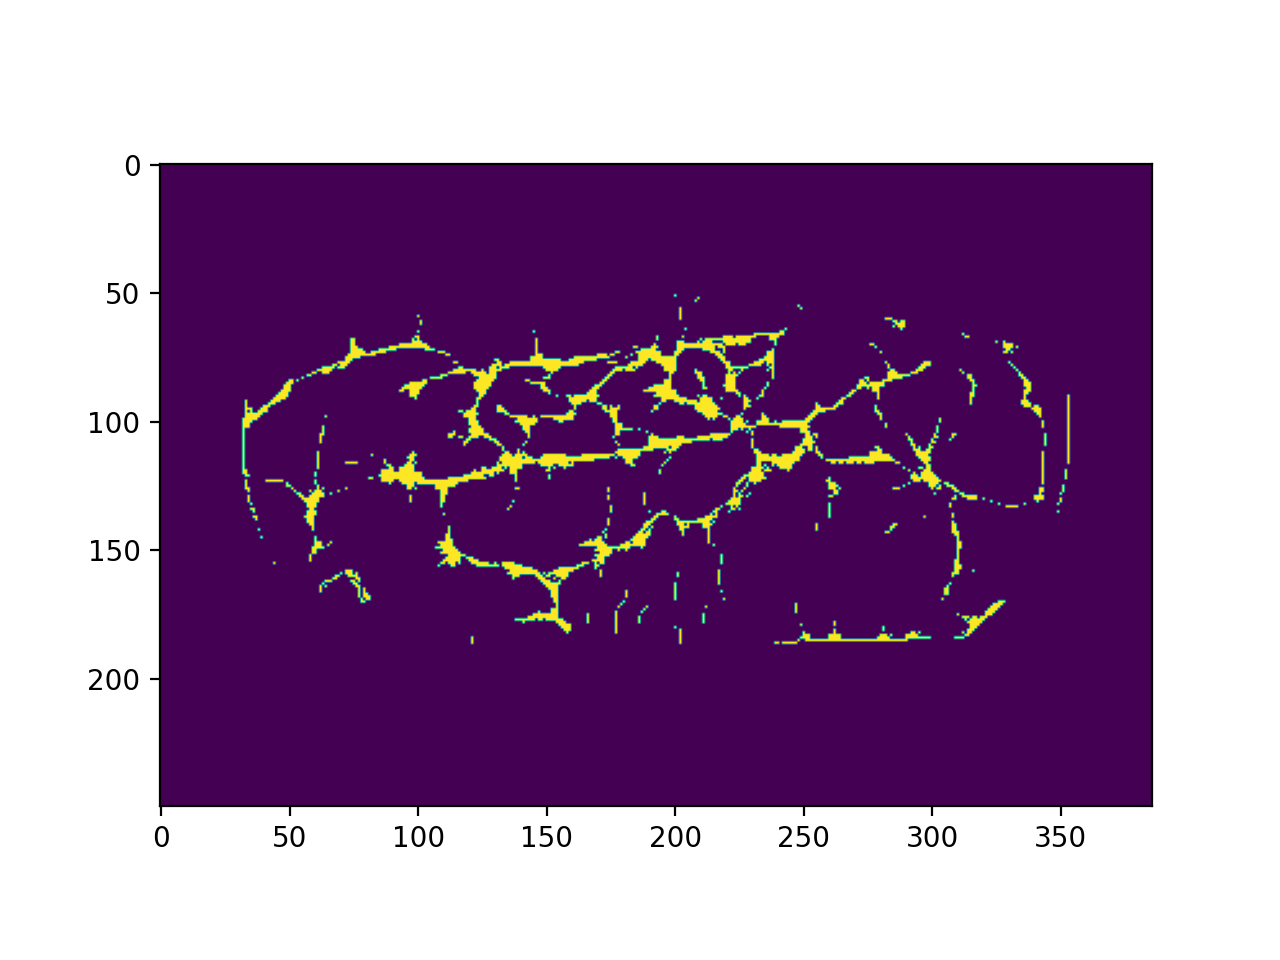
\includegraphics[width=.6\textwidth]{z.png}};
  \node[state,rectangle,minimum width=2.3cm,yshift=0cm, below of=B]           (A){Generate (\gen)};
  \node[text width=5.5cm,below of=A,yshift=0cm] (C) { $r, p$};
  
  \node[text width=5.5cm,right of =B, xshift=2.5cm] (D) {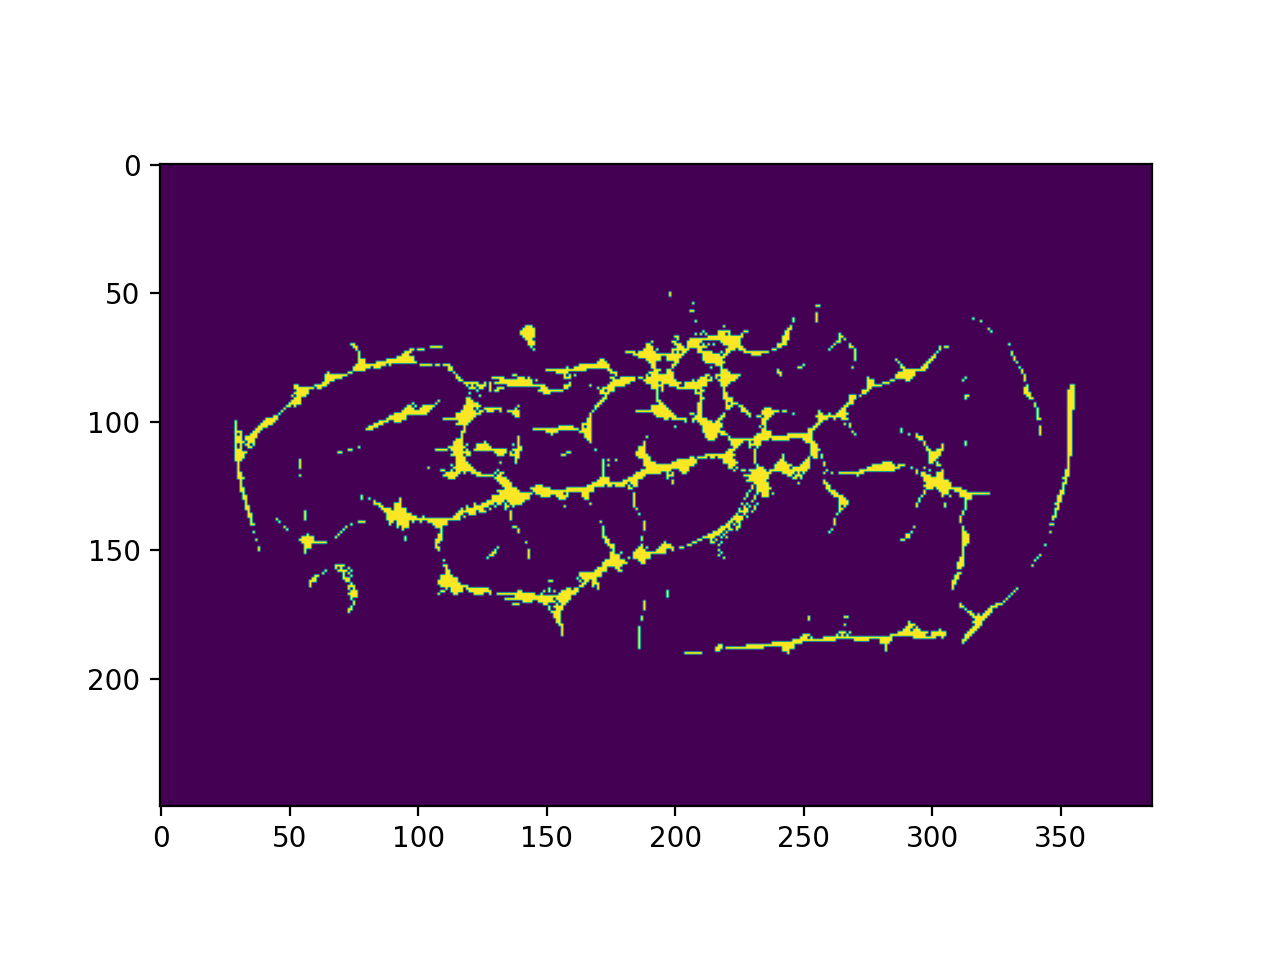
\includegraphics[width=.6\textwidth]{z2.png}, $p$};
  \node[state,rectangle,minimum width=2.3cm,yshift=0cm, below of=D]           (E){Reproduce (\rep)};
  \node[text width=5.5cm,below of=E,yshift=0cm] (F) {$\bot$};  
  
  \node[text width=5.5cm, right of =E,xshift=1.2cm] (G) {$\dots$};
  
  \node[state,rectangle,minimum width=2.3cm,yshift=0cm, right of=G, xshift=1.2cm]           (H){Reproduce (\rep)};
  \node[text width=5.5cm,below of=H,yshift=0cm] (J) {$r$};  \node[text width=5.5cm,above of =H] (I) {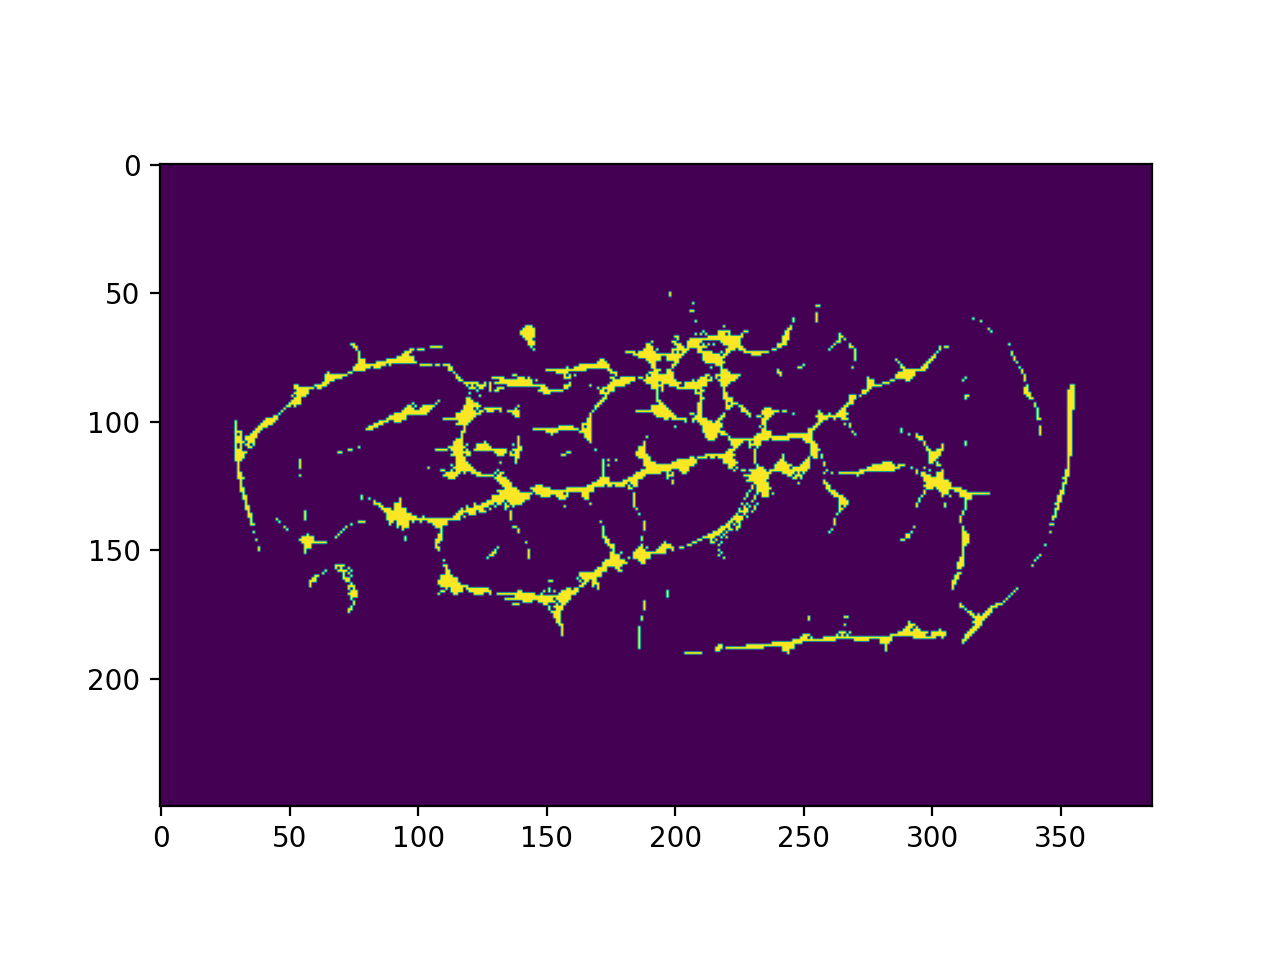
\includegraphics[width=.6\textwidth]{z2.png}, $p$};
  
  
    \path[->,draw]
    (B) edge node[] {} (A)
    (A) edge node[] {} (C)
    (D) edge node[] {} (E)
    (E) edge node[] {} (F)
    (I) edge node[] {} (H)
    (H) edge node[] {} (J);
}

\end{tikzpicture}
\end{figure}\pause

\textit{Disadvantage:} may require a large number of transformations \& may not be possible to have unlimited calls, e.g., log-in to website
\end{frame}
%------------------------------------------------
\begin{frame}{Outline}
   \begin{enumerate}
   \item Find a suitable \fe construction
\begin{enumerate}
    \item Wish-list
    \item The construction
    \item Parameter estimation\\
\end{enumerate}
   \item Data has noise
   \begin{enumerate}
       \item Access to the model \& probe
       \item Access to multiple instances of \rep
       \item \textbf{Access to a single instance of \rep}
        \begin{enumerate}
            \item Alignment methods (4)
            \item Evaluation
        \end{enumerate}
   \end{enumerate}    
\end{enumerate} 
\end{frame}

%------------------------------------------------
\begin{frame}{Access to a single instances of \rep}
$method_1$: shift the image such that its centre of mass becomes the physical centre of the image\\~\pause

$method_2$: shift on $y$-axis and rotate according to the line parameters that pass through the column-wise centre of the finger contour\\~\pause


$method_3$: $method_2$ + shift on $x$-axis using the position of the fingertip\\~\pause
% (first right-most edge of the mask with sufficiently many points) 

$method_4$: shift on $x$-axis using the left-most edge %(first edge of the mask with sufficiently many points) %localise position $i$ on the $x$-axis as the first edge of the mask with sufficiently many points and shift on $x$-axis by $ct_x - i$ where $ct_x$ is a constant value

\end{frame}
%------------------------------------------------
\begin{frame}{Outline}
   \begin{enumerate}
   \item Find a suitable \fe construction
\begin{enumerate}
    \item Wish-list
    \item The construction
    \item Parameter estimation\\
\end{enumerate}
   \item Data has noise
   \begin{enumerate}
       \item Access to the model \& probe
       \item Access to multiple instances of \rep
       \item Access to a single instance of \rep
        \begin{enumerate}
            \item Alignment methods (4)
            \item \textbf{Evaluation}
        \end{enumerate}
   \end{enumerate}    
\end{enumerate} 
\end{frame}
%------------------------------------------------
\begin{frame}{Evaluation}
    \begin{table}[t]
\tiny
    \centering
    \begin{tabular}{c|c|c|c|c|c|c}
         $pair$ & $none$ & $method_1$ &  $method_2$ & $method_3$ & $method_4$ & $optimal$ \\
         \hline
0  & 0.070191 & 0.073493 & 0.072404 & 0.072404 & \textbf{0.06988} & 0.063298 \\
1  & 0.070623 & 0.071288 & \textbf{0.06715} & \textbf{0.06715} & 0.071243 & 0.062932 \\
2  & 0.06516 & 0.071875 & \textbf{0.067223} & 0.067969 & 0.069127 & 0.063608 \\
3  & 0.059453 & 0.069515 & 0.064984 & 0.064984 & \textbf{0.059652} & 0.058943 \\
4  & 0.069902 & 0.072496 & \textbf{0.069326} & \textbf{0.069326} & 0.070855 & 0.070058 \\
5  & 0.063032 & 0.068728 & \textbf{0.065389} & \textbf{0.065389} & 0.067154 & 0.063254 \\
6  & 0.069714 & \textbf{0.067609} & 0.067617 & 0.068301 & 0.069714 & 0.066013\\
7  & 0.061126 & 0.066622 & \textbf{0.061565} & \textbf{0.061565} & 0.064162 & 0.061126 \\
8  & 0.082491 & 0.083134 & \textbf{0.081067} &  0.08144 & 0.081715 & 0.079743 \\
9  & 0.087212 & 0.097762 & 0.089482 & \textbf{0.087326} & 0.089849 & 0.075598 \\
10  & 0.082214 & 0.084541 & \textbf{0.079202} & \textbf{0.079202}  & 0.080929 & 0.078092 \\
11  & 0.077183 & 0.084342 & 0.077648 & 0.077648 & \textbf{0.077183} & 0.066102 \\
12  &  0.083566 & 0.083078 & \textbf{0.079513} & \textbf{0.079513} & 0.08463 & 0.073681 \\
13  & 0.086469 & 0.087844 & \textbf{0.08713} & \textbf{0.08713} & 0.088952 & 0.081704 \\
14  & 0.071609 & 0.072451 & 0.072539 & 0.072539 & \textbf{0.071609} & 0.061325 \\
15  &  0.077405 & 0.078579 & \textbf{0.074653} & \textbf{0.074653} & 0.075609 & 0.068739 \\
16  & 0.057502 & 0.063952 & \textbf{0.054995} & 0.05514 & 0.057746 & 0.053557 \\
17  & 0.097418 & 0.09693 & \textbf{0.094995} & 0.095057 & 0.097662 & 0.093562 \\
18  & 0.084752 & 0.084087 & \textbf{0.082332} & \textbf{0.082332} & 0.084752 & 0.070944 \\
19  & 0.084752 & 0.08719 & \textbf{0.08344} & \textbf{0.08344} & 0.084198 & 0.08156
    \end{tabular}
    \caption{Hamming distance between the model and probe. $none$ indicates no image transformation for neither the model nor the probe while $optimal$ shifts only the probe by the coordinates $(x,y)$ obtained from \textit{miurascore}. In bold we highlight the best method, i.e., $\min_i(method_i - optimal) = \min_i(method_i - none) = \min_i(method_i)$.}
    \label{tab:hdms}
\end{table}
\end{frame}
%------------------------------------------------
\begin{frame}{Conclusion}
\begin{enumerate}
   \item Find a suitable \fe construction
   \begin{itemize}
       \item \rfe [CFP$^{+}$16]
       \item Biometric hashing to handle assumptions on source
       \item $k=40$, $f=3.2 \times 10^9$\\~
   \end{itemize}

   \item Data has noise
   \begin{itemize}
       \item $method_2$, i.e., translation on $y-$axis and rotation, to minimise misalignment between the model \& probe
   \end{itemize}
    
\end{enumerate} 
\end{frame}

%------------------------------------------------
\begin{frame}{Future work}
Given a larger dataset $D$:
\begin{itemize}
    \item Estimate the entropy for $D$ and (possibly different) feature extraction method(s)~\pause
    \item Estimate parameters for the construction\\~\pause
\end{itemize}

Different ways to fulfil the assumptions on source, e.g., feature extraction, restrict to an area of interest\\~\pause

Consider image transformation using access to the model\\~\pause
% This can consequently have a positive impact on the mean error rate and the parameters of \fe constructions.

\centering \large\textcolor{dred}{Thank you!}
\end{frame}
%------------------------------------------------
\end{document}